\chapter{Proof-of-Concept}%
\label{ch:poc}
Voor het eerste praktische deel van deze bachelorproef werden er drie virtuele machines opgezet binnen VirtualBox met behulp van Vagrant om een gecontroleerde testomgeving te creëren. Deze virtuele machines (VM’s) simuleren een scenario waarin een ransomware-aanval gericht wordt op databases die door het bedrijf worden beheerd. Het primaire doel van deze simulatie is aan te tonen dat het gebruik van immutable storage een effectieve maatregel kan zijn om belangrijke data te beschermen tegen ransomware-aanvallen.
\subsection{Relevantie van de PoC voor de Azure-omgeving van Forvis Mazars}
De Proof-of-Concept (PoC) in VirtualBox simuleert een ransomware-aanval in een lokale omgeving, gericht op het evalueren van beveiligingsmaatregelen zoals immutable storage. Deze aanpak sluit nauw aan bij de Azure-omgeving van Forvis Mazars, waar databases en back-ups worden beheerd.

De technieken uit de PoC, zoals immutable storage, kunnen direct worden toegepast in Azure via functies zoals immutable blobs in Azure Storage. Dit maakt het mogelijk om gegevens beter te beschermen tegen wijzigingen of verwijdering. Daarnaast biedt de PoC een veilig platform om de impact van een ransomware-aanval te begrijpen en te testen hoe snel en effectief back-ups kunnen worden hersteld, wat een cruciaal aspect is voor de bedrijfscontinuïteit.

Forvis Mazars kan de PoC gebruiken om risico’s te analyseren en beveiligingsoplossingen eerst kleinschalig te testen, alvorens deze op grotere schaal binnen hun cloudinfrastructuur toe te passen. Hiermee helpt de PoC bij het verfijnen en optimaliseren van hun bestaande Azure-back-upstrategie.
\subsection{Technische uitwerking}
Voor het opzetten van de virtuele machines in de Proof-of-Concept (PoC) werd gebruik gemaakt van een Vagrantfile. De Vagrantfile definieert de specificaties en configuraties van de VM’s, zoals geheugen, CPU, netwerkadapters en besturingssysteem. 
\begin{lstlisting}[language=Ruby, caption={Vagrantfile voor drie VM's: Back-up Server, Client, en Attacker}]
Vagrant.configure("2") do |config|

# Primary VM
config.vm.define "primary" do |primary|
primary.vm.box = "ubuntu/jammy64"

primary.vm.network "private_network", ip: "192.168.0.10", virtualbox__intnet: "internal_network"

primary.vm.provider "virtualbox" do |vb|
vb.memory = "2048" 
vb.cpus = 1        
end
end

# Back-up VM
config.vm.define "backup" do |backup|
backup.vm.box = "ubuntu/jammy64"

backup.vm.network "private_network", ip: "192.168.0.20", virtualbox__intnet: "internal_network"

backup.vm.provider "virtualbox" do |vb|
vb.memory = "2048" 
vb.cpus = 1       
end
end

# Attacker VM
config.vm.define "attacker" do |attacker|
attacker.vm.box = "ubuntu/jammy64"

attacker.vm.network "private_network", ip: "192.168.0.30", virtualbox__intnet: "internal_network"

attacker.vm.provider "virtualbox" do |vb|
vb.memory = "1024" 
vb.cpus = 1        
end
end

end
\end{lstlisting}

In de onderstaande tabel worden de specificaties van de drie virtuele machines weergegeven die in de Proof-of-Concept zijn gebruikt. Elke VM heeft een specifieke functie binnen het netwerk. De tabel bevat details over de hoeveelheid toegewezen RAM, het aantal CPU-cores, het gebruikte besturingssysteem, de toegewezen IP-adressen en de configuratie van de netwerkadapter. Deze configuratie zorgt ervoor dat de VM's binnen hetzelfde interne netwerk met elkaar kunnen communiceren, wat essentieel is voor het testen van de ransomware-aanval en de back-upstrategieën.
\begin{longtable}{|l|c|c|c|l|l|}
    \hline
    \textbf{Functie} & \textbf{RAM} & \textbf{CPU Cores} & \textbf{IP} & \textbf{Besturingssysteem} & \textbf{Netwerkadapter} \\ \hline
    Primary server    & 2 GB         & 1                  & 192.168.0.10 & Ubuntu 22.04.5 LTS & NAT + Internal \\ \hline
    Back-up server           & 1 GB         & 1                  & 192.168.0.20 & Ubuntu 22.04.5 LTS & NAT + Internal \\ \hline
    Attacker VM         & 2 GB         & 1                  & 192.168.0.30 & Ubuntu 22.04.5 LTS     & NAT + Internal \\ \hline
    
\caption{Beschrijving van de virtuele machines in de Proof of Concept}
\end{longtable}

De Primary VM stelt een actieve databankserver voor binnen een bedrijfsomgeving. Deze server bevat de operationele data van het bedrijf en vertegenwoordigt de belangrijkste bron die beschermd moet worden tegen dataverlies of aanvallen. 

De Back-up VM fungeert als een back-upserver waarop regelmatig de databankback-ups worden opgeslagen. Deze back-upserver is cruciaal voor bedrijfscontinuïteit en disaster recovery, omdat ze in geval van een aanval of fout de herstelmogelijkheden biedt. 

De Attacker VM vertegenwoordigt een hacker met slechte intenties binnen de testomgeving. Deze machine wordt gebruikt om een ransomware-aanval te simuleren, waarbij de functionaliteit van zowel de Primary VM als de Back-up VM wordt bedreigd. Het doel van deze opstelling is om te demonstreren hoe een back-upstrategie, inclusief technieken zoals immutable storage, een bedrijf kan beschermen tegen de gevolgen van een dergelijke aanval.
\subsubsection{Aanmaken van de database}
Op de primary VM werd een eenvoudige SQL-database geïnstalleerd en de volgende tabel aangemaakt om als testdata te dienen:
\begin{lstlisting}[language=SQL, caption={MySQL-code voor het aanmaken van de testdatabank}]
CREATE TABLE employees (
    id INT AUTO_INCREMENT PRIMARY KEY,
    name VARCHAR(50),
    role VARCHAR(50)
);
INSERT INTO employees (name, role) VALUES 
    ('Alice', 'Engineer'), 
    ('Bob', 'Manager'), 
    ('Charlie', 'Analyst');
\end{lstlisting}



\subsubsection{Back-up van de database}
Nadien werd de database geëxporteerd naar een \texttt{.sql}-bestand met het volgende \texttt{mysqldump}-commando:
\begin{lstlisting}[language=script, caption={mysqldump commando om een databank te exporteren}]
mysqldump -u testuser -p testdb > /home/vagrant/backup.sql
\end{lstlisting}
Het resulterende bestand, \texttt{backup.sql}, werd vervolgens met BorgBackup opgeslagen in een back-uprepository op de back-up VM. De repository werd vooraf geïnitialiseerd met het volgende commando:
\begin{lstlisting}[language=script, caption={Borg commando om een map te initialiseren als Borg repository}]
borg init --encryption=repokey /home/vagrant/backups
\end{lstlisting}
Vervolgens werd de back-up gemaakt:
\begin{lstlisting}[language=script, caption={Borg commando om een back-up te nemen}]
borg create --progress 
ssh://vagrant@192.168.0.20/home/vagrant/backups::backup-$(date +%Y-%m-%d) 
/home/vagrant/backup.sql
\end{lstlisting}

\subsubsection{Beveiliging van de back-updirectory}
Om de back-updirectory ransomware-resistent te maken, werd het Linux-commando \texttt{chattr} gebruikt om het \textit{immutable}-attribuut toe te passen op de back-updirectory. Dit attribuut zorgt ervoor dat er geen wijzigingen aan de bestanden in de directory gebeuren, zelfs door gebruikers met \texttt{root}-rechten. Het commando:
\begin{lstlisting}[language=script, caption={Linux commando om de map immutable te maken}]
sudo chattr +i /home/vagrant/backups/
\end{lstlisting}

\subsubsection{Simulatie van de ransomware-aanval}
Op de attacker VM werd een script gebruikt om de ransomware-aanval te simuleren. Het script probeert alle bestanden in de back-updirectory te hernoemen door \texttt{.malware} toe te voegen aan de bestandsnamen. Dit zou overeenkomen met een ransomware-aanval waarbij de back-up bestanden geëncrypteerd worden. Het script is hieronder weergegeven:
\begin{lstlisting}[language=script, caption={Bash script om een ransomware-aanval na te bootsen}]
#!/bin/bash
    
BACKUP_DIR="/home/vagrant/backups"
    
for file in "$BACKUP_DIR"/*; do
  if [ -f "$file" ]; then
    if mv "$file" "${file}.malware"; then
      echo "Renamed $file to ${file}.malware"
    else      
      echo "Error: Could not rename $file"    
    fi    
  fi    
done    
\end{lstlisting}
Voor het gemak heeft de Attacker VM volledige controle gekregen over de Back-up VM. Dit is gedaan omdat de scope van deze bachelorproef niet is om toegang te verkrijgen tot een server, maar eerder om een gecontroleerde omgeving te creëren waarin een Attacker VM een ransomware-aanval nabootst. Het doel is te demonstreren hoe de ransomware zich verspreidt naar de back-up directory, en niet om de daadwerkelijke methoden voor het verkrijgen van toegang tot een server in detail uit te werken.

Toen dit script werd uitgevoerd op de back-up VM, werd duidelijk dat het hernoemen van de bestanden niet lukte vanwege het immutable-attribuut. Dit toont aan dat de ransomware-aanval niet slaagde en de bestanden in de back-updirectory beschermd bleven.

\subsubsection{Herstellen van de back-ups}
Om te bewijzen dat de back-ups nog steeds bruikbaar waren, werd een herstelproces uitgevoerd op de primary VM vanuit de Borg-repository:
\begin{lstlisting}[language=script, caption={Borg commando om een back-up te herstellen}]
borg extract 
ssh://vagrant@192.168.0.20/home/vagrant/backups::backup-2024-12-05
\end{lstlisting}

De databank werd opnieuw opgezet vanuit het bestand dat uit de Borg-repository werd gehaald met het volgende commando:
\begin{lstlisting}[language=script, caption={MySQL commando om een databank te herstellen vanuit een .sql-bestand}]
mysql -u root -p restored_db < /home/vagrant/backup.sql
\end{lstlisting}
De back-up werd gebruikt om de database te herstellen en te controleren. Het herstelproces verliep succesvol, wat bewijst dat de immutable storage de integriteit van de back-ups had behouden en dat de bestanden veilig waren gebleven ondanks de ransomware-aanval.

\newpage
\subsection{Implementatie van immutable storage in de Azure-omgeving}
\subsubsection{Aanmaken van een storage account}
De eerste stap in het implementeren van Immutable Storage in Azure is het aanmaken van een \texttt{Storage Account} in de Azure Portal. 
\begin{figure}[h]
    \centering
    \captionsetup{justification=centering}    
    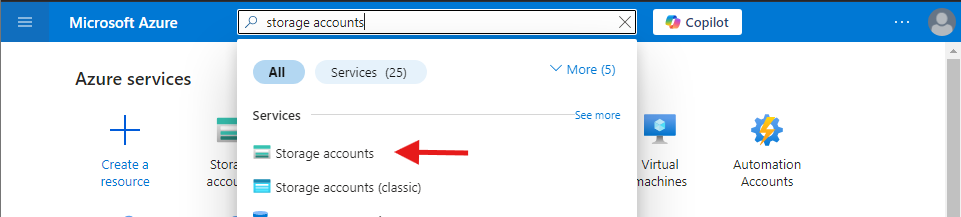
\includegraphics[width=0.8\textwidth]{img/1imm.png}
    \caption{Storage account zoekopdracht binnen de Azure Portal}
\end{figure}
Bij het aanmaken van het storage account kiezen we de correcte resource group, naam die het account moet krijgen, regio en bij redundancy kiezen we voor \texttt{Locally-redundant storage (LRS)}. Bij de optie \texttt{Account kind} kiezen we voor \texttt{General-purpose v2}, omdat deze versie alle benodigde functionaliteit biedt, zoals het ondersteunen van de blob storage en het configureren van immutability policies. 
\begin{figure}[h]
    \centering
    \captionsetup{justification=centering}    
    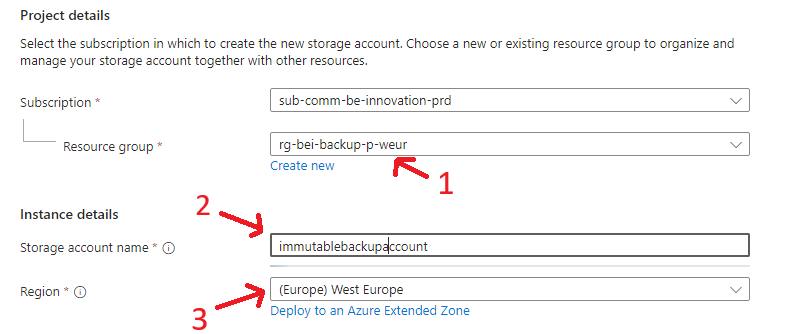
\includegraphics[width=0.8\textwidth]{img/3.1imm.png}
    \caption{Configuratie voor het nieuwe storage account}
\end{figure}
\begin{figure}[h]
    \centering
    \captionsetup{justification=centering}    
    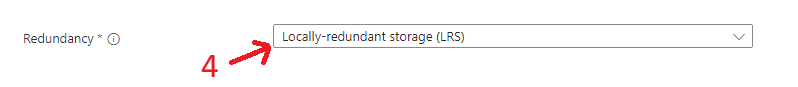
\includegraphics[width=0.8\textwidth]{img/3.2imm.png}
    \caption{Tweede deel van de configuratie voor het nieuwe storage account}
\end{figure}
\newpage
\subsubsection{Aanmaken van een container binnen het storage account}
Na het aanmaken van het storage account moet er een container geconfigureerd worden binnen het nieuwe storage account om de gegevens op te slaan. Bij het aanmaken van de container moet de \texttt{public access level} op private staan voor de veiligheid. Containers in Azure werken als mappen waarin je blobs kunt opslaan zoals back-ups.
\begin{figure}[h]
    \centering
    \captionsetup{justification=centering}    
    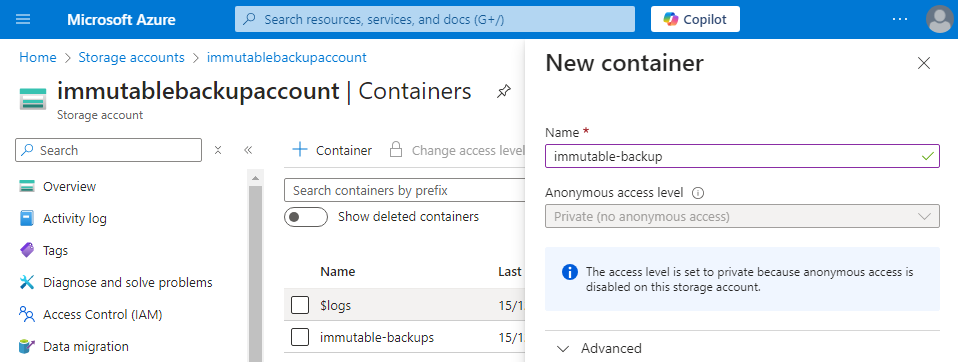
\includegraphics[width=0.8\textwidth]{img/4imm.png}
    \caption{Configuratie voor de container in het storage account}
\end{figure}
\subsubsection{Opzetten van een time-based retention policy}
Nadien moet er een immutability policy opgezet worden. Hierbij werd gekozen voor een time-based retention policy van 90 dagen, de back-up is met andere woorden bescherm tegen verwijdering of wijziging voor deze periode. Dit is een veilige en praktische keuze voor back-ups. Daarnaast is er bij de optie \texttt{ Allow protected append writes to } gekozen voor \texttt{ Block and append blobs}, dit maakt het mogelijk om gegevens te blijven toevoegen aan de blob zonder de bestaande gegevens te wijzigen of te verwijderen, wat ideaal is voor scenario's zoals logbestanden of incrementele back-ups.
\begin{figure}[h]
    \centering
    \captionsetup{justification=centering}    
    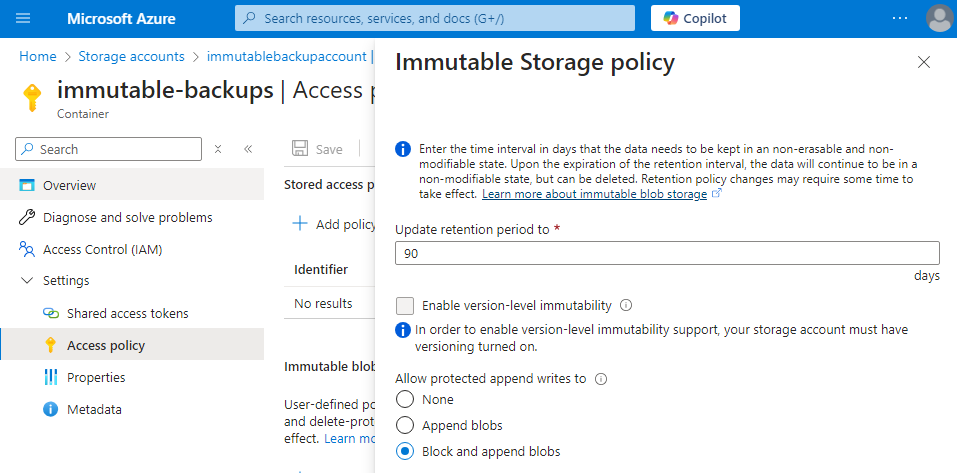
\includegraphics[width=0.8\textwidth]{img/6imm.png}
    \caption{Configuratie voor time-based retention policy}
\end{figure}
\newpage
\subsubsection{Testen van de immmutable storage}
Om de immutable storage te testen is er gekozen om een back-up van een MySQL-database de uploaden naar de container. Na het uploaden van het bestand was er geen optie om dit bestand te verwijderen of te wijzigen. Met andere woorden is deze back-up dus beschermd tegen een ransomware-aanval.
\begin{figure}[h]
    \centering
    \captionsetup{justification=centering}    
    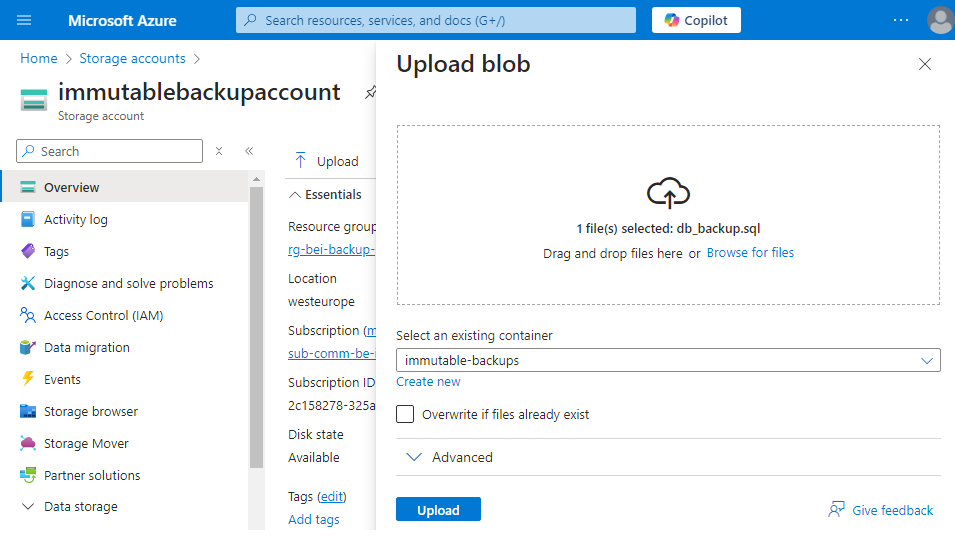
\includegraphics[width=0.8\textwidth]{img/7imm.png}
    \caption{Uploaden van het back-up bestand van de MySQL-databank}
\end{figure}
\begin{figure}[h]
    \centering
    \captionsetup{justification=centering}    
    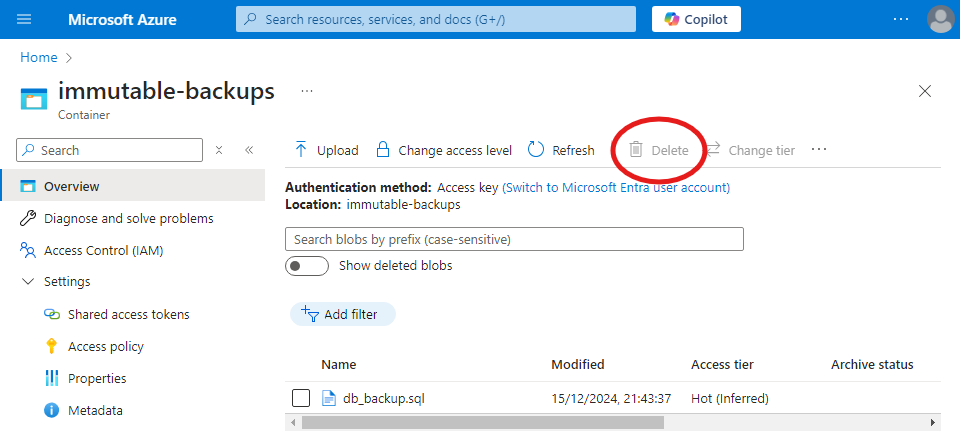
\includegraphics[width=0.8\textwidth]{img/8imm.png}
    \caption{Screenshot van de poging om het bestand te verwijderen, waarbij de actie wordt geblokkeerd}
\end{figure}
\subsubsection{Conclusie}
De implementatie van immutable storage op het azure storage account is succesvol afgerond, waardoor de opgeslagen back-ups nu beschermd zijn tegen onverwachte wijzigingen of verwijderingen. Daarnaast worden er dagelijks automatische back-ups van de databanken genomen, welke een retentieperiode van 7 dagen hebben. Dit zorgt ervoor dat er altijd een versie van de back-up beschikbaar is, zelfs als de meest recente back-up beschadigd of onbruikbaar blijkt. Deze combinatie van immutable storage en versiebeheer versterkt de bescherming tegen dataverlies en maakt het mogelijk om eerdere, werkende back-ups snel te herstellen.


\subsection{Automatiseren van de manuele back-ups met Docker en Python}
\subsubsection{Overzicht van de oplossing}
Om een efficiënte en schaalbare oplossing te bieden voor het maken van databaseback-ups, werd een geautomatiseerd systeem ontwikkeld met behulp van een Python-script en een Docker-container. Dit systeem automatiseert zowel het maken van back-ups als het verwijderen van oude back-ups op basis van een ingestelde retentieperiode. De focus van deze implementatie is vooral herbruikbaarheid wat ervoor zorgt dat deze oplossing gemakkelijk geïmplementeerd kan worden in de productieomgeving van Forvis Mazars. Voor deze setup is er gebruik gemaakt van een databank die lokaal draait op een virtuele machine die als databank-server functioneert. Daarbij is er een Docker-container die, via het Python-script, back-ups neemt van de databank. Dit komt overeen met de actieve omgeving die Forvis Mazars gebruikt.

\subsubsection{Python-script voor back-ups}
Het Python-script vormt de kern van dit systeem en voert twee belangrijke taken uit. Enerzijds zorgt het voor het genereren van back-ups door gebruik te maken van \texttt{mysqldump} voor MySQL-databases en \texttt{pg\_dump} voor PostgreSQL-databases. Deze tools bieden de mogelijkheid om volledige databaseback-ups te maken die in een gestandaardiseerd formaat worden opgeslagen. Anderzijds implementeert het script een retentiebeleid waarbij oude back-ups die ouder zijn dan een vooraf ingestelde periode automatisch worden verwijderd. Daarnaast is logging geïntegreerd in het script om eventuele fouten of waarschuwingen te registreren, wat helpt bij monitoring en foutopsporing.

\subsubsection{Python-script: Backups en Retentie}
Het volledige Python-script is hieronder weergegeven:
\begin{lstlisting}[language=script, caption=Python-script voor back-ups en retentie]
import datetime
import os
import subprocess  # nosec
import argparse
import logging


class Backup:

def __init__(self, database_name, database_user, type, backup_dir):
timestr = datetime.datetime.now().strftime('%Y-%m-%d')
self.filename = f'backup-{type}-{timestr}-{database_name}.dump'
self.database_name = database_name
self.database_user = database_user
self.type = type
self.password = None
self.backup_dir = backup_dir
self.hostname_mysql = os.environ.get("HOSTNAME_MYSQL", "192.168.1.62")
self.hostname_psql = os.environ.get("HOSTNAME_PSQL", "192.168.1.62")
self.port_mysql = os.environ.get("PORT_MYSQL", "3306")
self.port_psql = os.environ.get("PORT_PSQL", "5432")

def set_password(self):
"""
Retrieve the database password from an environment variable.
"""
self.password = os.environ.get("DB_PASSWORD")
if not self.password:
logging.warning("Database password not set. Please provide the DB_PASSWORD environment variable.")
exit(1)

def create_backup(self, type):
"""
Create a backup of the database.
"""
# Ensure the backup directory exists
if not os.path.exists(self.backup_dir):
os.makedirs(self.backup_dir)

# Prepend the backup directory to the filename
full_path = os.path.join(self.backup_dir, self.filename)

if type == "MYSQL":
try:
cmd = [
'mysqldump',
'--single-transaction',
'-u', self.database_user,
f'-p{self.password}',
'-h', self.hostname_mysql,
'-P', str(self.port_mysql),
'--no-tablespaces',
'-B', self.database_name,
]

with open(full_path, 'w') as backup_file:
result = subprocess.run(cmd, stdout=backup_file, check=True)  # nosec

if result.returncode != 0:
logging.warning(f'Command failed. Return code: {result.returncode}')
exit(1)

return full_path

except Exception as e:
logging.warning(e)
exit(1)

elif type == "PSQL":
try:
cmd = [
'pg_dump',
'-U', self.database_user,
'-h', self.hostname_psql,
'-p', str(self.port_psql),
'-F', 'c',
'-f', full_path,
self.database_name
]

result = subprocess.run(cmd, check=True)  # nosec

if result.returncode != 0:
logging.warning(f'Command failed. Return code: {result.returncode}')
exit(1)

return full_path

except Exception as e:
logging.warning(e)
exit(1)

@staticmethod
def delete_old_backups(directory, retention_days):
"""
Deletes backup files older than the specified retention period.
"""
now = datetime.datetime.now()
logging.info(f"Starting cleanup of backups in {directory} with retention period: {retention_days} days")
for file in os.listdir(directory):
if file.startswith("backup-") and file.endswith(".dump"):
file_path = os.path.join(directory, file)
file_mtime = datetime.datetime.fromtimestamp(os.path.getmtime(file_path))
age = (now - file_mtime).days
logging.info(f"Checking file {file_path}: age = {age} days")
if age >= retention_days:
try:
os.remove(file_path)
logging.info(f"Deleted old backup: {file_path}")
except Exception as e:
logging.warning(f"Failed to delete {file_path}: {e}")
else:
logging.info(f"File {file_path} is not old enough to delete (age = {age} days).")


def main():
# Configure logging
logging.basicConfig(
level=logging.INFO,
format="%(asctime)s - %(levelname)s - %(message)s"
)

parser = argparse.ArgumentParser(description="Execute a local backup of a database.")
parser.add_argument("-dn", "--database_name", required=True, help="Enter the name of the database for the backup.")
parser.add_argument("-du", "--database_user", required=True, help="Enter the username of the database for the backup.")
parser.add_argument("-b", "--backup", action="store_true", help="Backup the database.")
parser.add_argument("-t", "--type", choices=["MYSQL", "PSQL"], required=True, help="MYSQL or PSQL")
parser.add_argument("-bd", "--backup_dir", default=".", help="Directory where backups are stored.")
parser.add_argument("-r", "--retention", type=int, help="Retention period in days for keeping backups.")
args = parser.parse_args()

db_name = args.database_name
db_user = args.database_user
backup = args.backup
type = args.type
backup_dir = args.backup_dir
retention = args.retention

if backup:
b = Backup(db_name, db_user, type, backup_dir)
try:
b.set_password()
backup_file = b.create_backup(type=type)
except Exception as e:
logging.warning(e)
else:
logging.info(f"Backup successful: {backup_file}")

if retention is not None:
try:
Backup.delete_old_backups(directory=backup_dir, retention_days=retention)
logging.info(f"Old backups older than {retention} days were successfully deleted from {backup_dir}.")
except Exception as e:
logging.warning(f"Failed to clean up old backups: {e}")


if __name__ == '__main__':
main()

\end{lstlisting}

\subsubsection{Automatisering met Docker}
De automatisering wordt verder versterkt door het gebruik van een Docker-container. Deze container biedt een reproduceerbare omgeving waarin het script kan worden uitgevoerd. Door een gestandaardiseerde Docker-image te gebruiken die gebaseerd is op Ubuntu, wordt een consistente setup gegarandeerd dat Forvis Mazars makkelijk kan implementeren. Binnen de container wordt een \texttt{setup.sh} script uitgevoerd om cronjobs te configureren die verantwoordelijk zijn voor het dagelijks maken van nieuwe back-ups om 2:00 uur 's nachts en het verwijderen van oude back-ups die ouder zijn dan 14 dagen. De retentieperiode is hier dus op 14 dagen gezet voor de dagelijkse back-ups. Daarnaast zorgt dit Bash-script ook voor het opstarten van de cron-service. Dit is nodig om een cronjob uit te voeren. De back-ups worden opgeslagen in een aparte directory binnen de container, en de cron-service wordt gestart door het setup-script. Bij het opzetten van de container  worden ook alle benodigde softwarepakketten geïnstalleerd zoals \texttt{mysql-client}, \texttt{cron}, en \texttt{python3}. Er worden 2 bestanden gekopieerd naar de container namelijk het Python-script en het Bash-script.

\subsubsection{Dockerfile}
Hieronder volgt de Dockerfile die gebruikt is voor het bouwen van de container:
\begin{lstlisting}[language=Dockerfile, caption=Dockerfile voor de back-upcontainer]
FROM ubuntu:latest

WORKDIR /src

USER root
RUN apt update -y \
&& apt -y install mysql-client postgresql-client cron nano \
&& apt install -y python3

COPY src/* /src/
COPY crontab.txt /etc/cron.d/my-cron-job
COPY src/setup.sh /src/setup.sh

RUN chmod 0644 /etc/cron.d/my-cron-job && \
chmod +x /src/backup_script.py 
RUN chmod +x /src/setup.sh
ENTRYPOINT ["tail"]
CMD ["-f", "/dev/null"]
\end{lstlisting}

\subsubsection{Setup-script}
Het \texttt{setup.sh}-script dat wordt uitgevoerd in de container is hieronder weergegeven:
\begin{lstlisting}[language=script, caption=Setup-script voor het configureren van cronjobs]
#!/bin/bash
service cron start

mkdir /src/backups

echo -e "* * * * * DB_PASSWORD=root PGPASSWORD=root python3 /src/backup_script.py -dn testdb -du root -t MYSQL -b -bd /src/backups >> /var/log/cron.log 2>&1\n* * * * * DB_PASSWORD=root PGPASSWORD=root python3 /src/backup_script.py -dn testdb -du root -t PSQL -b -bd /src/backups >> /var/log/cron.log 2>&1\n0 2 * * * DB_PASSWORD=root PGPASSWORD=root python3 /src/backup_script.py -bd /src/backups -r 14 -dn testdb -du root -t MYSQL >> /var/log/cron.log 2>&1" | crontab -

exec "$@"
\end{lstlisting}

\subsubsection{Relevantie voor Forvis Mazars}
Deze oplossing kan eenvoudig worden geïntegreerd in de infrastructuur van Forvis Mazars, omdat het gebruik maakt van Docker-containers. Forvis Mazars beheert hun back-ups binnen een Kubernetes-cluster, en Docker-containers kunnen rechtstreeks als pods worden gedeployed in Kubernetes. Hierdoor kan de huidige oplossing zonder aanpassingen worden hergebruikt. De setup in deze implementatie, waarbij de databases op een virtuele machine draaien en de back-ups worden uitgevoerd via Docker-containers, komt overeen met de werkomgeving van Forvis Mazars. Dit zorgt ervoor dat de voorgestelde oplossing naadloos aansluit op hun huidige infrastructuur en gebruiksbehoeften.


\subsection{Herstelcapaciteit (Restore from Backup)}
Een belangrijk onderdeel van het praktijkgedeelte van dit onderzoek is het testen van de \textbf{herstelcapaciteit} (Restore from Backup). Dit was een essentiële vereiste in het onderzoek, waarbij de focus lag op het efficiënt en snel herstellen van systemen vanuit de back-ups. Het doel was om een idee te krijgen over hoe snel en betrouwbaar een databank up-and-running kan zijn na het ondergaan van een incident.

\subsubsection{Toepassing van de Herstelstrategie}
Om deze must-have te evalueren, heb ik de gehele herstelprocedure in een gecontroleerde testomgeving uitgevoerd. Deze testomgeving komt grotendeels overeen met de actieve omgeving die Forvis Mazars gebruikt. Dit proces omvatte de volgende stappen:

\begin{enumerate}
    \item \textbf{Back-ups ophalen uit de immutable storage in Azure} \\
    De back-ups werden veilig opgeslagen in een Azure Storage Account met een immutable opslagbeleid, wat een cruciale maatregel is tegen ransomware-aanvallen. Door het gebruik van het \texttt{az storage blob download}-commando werden de back-ups gedownload naar de lokale virtuele machine.
    
    \item \textbf{Herstellen van de PostgreSQL- en MySQL-databanken} \\
    Na het downloaden werden de PostgreSQL- en MySQL-databases opnieuw opgezet met herstelcommando’s. Voor PostgreSQL werd het bestand hersteld met \texttt{pg\_restore}, terwijl voor MySQL gebruik werd gemaakt van het \texttt{mysql}-commando. Beide hersteltaken verliepen succesvol en zonder dataverlies, waarmee de betrouwbaarheid van de back-upstrategie werd aangetoond. Dit hele proces is gemeten en duurde ongeveer \textbf{23 seconden}, wat wijst op een snelle toegang tot de back-ups in noodsituaties.
\end{enumerate}

\subsubsection{Link met Herstelcapaciteit}
De testprocedure toont aan dat de opgestelde back-upstrategie niet alleen effectief is in het beschermen van gegevens, maar ook voldoet aan de eisen van herstelcapaciteit:

\begin{itemize}
    \item \textbf{Efficiëntie:} Het herstelproces, vanaf het downloaden van de back-ups tot het opnieuw opzetten van de databases, verliep in een relatief korte tijd. Dit bevestigt dat de back-ups eenvoudig en snel toegankelijk zijn, wat essentieel is in een bedrijfsomgeving waar down-time zo laag mogelijk moet zijn.
    
    \item \textbf{Betrouwbaarheid:} Door gebruik te maken van immutable opslag in Azure worden de back-ups beschermd tegen ongewenste acties en aanvallen, wat de kans op succesvol herstel sterk verhoogt.
\end{itemize}

\subsubsection{Conclusie}
De uitgevoerde tests bieden waardevolle inzichten in de herstelcapaciteit van de back-upstrategie. Het toont aan hoe een goed ontworpen back-upplan bedrijven in staat stelt om snel te reageren op noodsituaties en hun systemen betrouwbaar te herstellen. Hiermee is aangetoond dat het systeem niet alleen beschermt tegen gegevensverlies, maar ook operationeel herstel mogelijk maakt binnen een acceptabele tijd. Dit maakt het een reële oplossing voor bedrijven die ransomware-resistente back-upstrategieën willen implementeren.































